\chapter{Theoretical aspects}

\pagestyle{fancy}

\label{theoreticalAspects}

\section{Procedural Generation}

As already stated in the introduction, procedural generation is a method of generating content algorithmically. While mostly used for video games and animated movies, there are other fields where this method excels, such as city planning. Terrain and landscapes, textures, materials, meshes, even loot systems and non playable character (NPC) dialogue can be machine-generated. The core idea is telling the computer to produce certain results, based on some kind of randomness. As true randomness only occurs in the real world, one example being cosmic background radiation, programmers have to rely on what they call pseudo-random numbers. These numbers could be, for example, $\pi$ digits, with the values picked from a certain point, called \textit{seed}.\cite{procgenwiki}.\\

The element of randomness that the procedural generation offers is something that game developers can fully take advantage of to keep the players engaged by creating interesting, highly re-playable levels. The game \textit{Rouge}, published in 1980 is a classic example of a successful game that uses algorithms to generate its content. It ended up defining an entire genre, under the name of \textit{rogue-like} games. Another interesting aspect of applications that heavily use procedural generation is the small file size, or \textit{footprint}. Due to the fact that almost everything is computer generated, there is no need of storing many assets on disk. For older games, this means files that take under one megabyte of data. That is quite impressive.\cite{freiknecht2017survey}.\\

Unfortunately, procedural generation has some limits, and very few big budget (AAA) games are fully based on this technique. Most of the times, developers use it to give a random feel to already existing, hand-made assets, or create unique customization options. For example, they might rotate the position of some buildings, or modify the colors of some armors. Most notably are computer generated loot systems, like the ones we see in the \textit{Borderlands} series. Since 2009, 4 games have been released in total under the title \textit{Borderlands}, every one of them featuring a captivating design aspect: randomized loot drops from enemies or chests. The element of surprise and excitement when a new item is given to the player is what keeps them motivated and engaged, resulting in a successful and long-lasting game series\cite{borderlands}.\\

Another area where generation algorithms start to really shine is music. Known as \textit{generative music}, this genre has been explored since 1956 (\textit{Push Button Bertha}). The term has been coined by \textit{Brian Eno}, who used procedural generation in many of his works, including \textit{Discreet Music (1975)}. Many artist are fascinated by the infinity aspect of this genre, while some just seek inspiration. In video games, the sound has to be specifically designed to match the player's state, actions and immerse him in a suitable atmosphere. Usually, the sound cues are directed by \textit{if statements}, mixing and blending different audio files to create the soundtrack that the player hears. When using a generative approach, the sounds are programmed to adapt fast to the input of the player and give him the audio responses he needs. Another important aspect is that this method is relatively cheap compared to AAA games such as Bethesda's \textit{Skyrim}, where orchestras and choirs recorded some, now well known, soundtracks\cite{collins2009introduction}.

\section{Procedural Noise}

\subsection{Overview}

In the world of computer graphics, procedural noise is one of the most successful techniques of achieving realistic artificial details. Mainly used in film production and for video games, noise algorithms gained popularity over the years, mainly thanks to \textit{Ken Perlin} and his research. In 1983, he developed the \textit{Perlin noise} function at \textit{Mathematical Applications Group, Inc. (MAGI)}, while working with \textit{The Walt Disney Company} at a science fiction action-adventure movie called \textit{Tron}. The idea came to him out of frustration with the machine-like look of computer-generated imagery\cite{perlinnoisewiki}. Later, in 1985, he officially documented his findings in a paper called \textit{An Image Synthesizer}\cite{perlin1985image} and was awarded an \textit{Academy Award for Technical Achievement} for creating the algorithm, which is still used today and included in many 3D computer graphics software like \textit{Blender} and \textit{Unity Engine}.\\

\begin{figure}[htp]
    \centering
    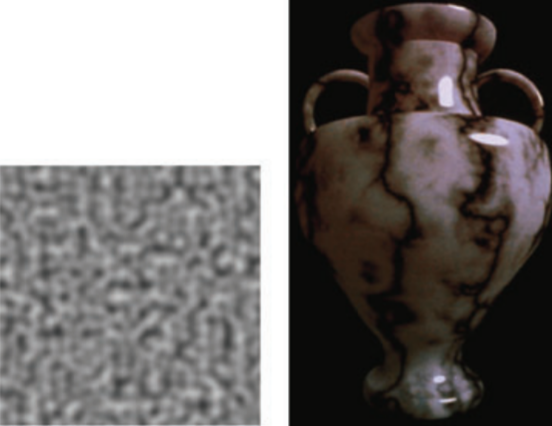
\includegraphics[width = 8cm]{figures/perlinMarbleVase.PNG}
    \caption{Perlin's procedural noise algorithm output (left) and his famous marble vase with one of the first procedurally generated textures (right).}
    \cite{perlin1985image}
    \label{fig:perlinMarbleVase}
\end{figure}

Noise can be intuitively defined as unstructured, random patterns that can be obtained using different mathematical functions and algorithms. It can be seen as “the random number generator of computer graphics”\cite{lagae2010survey}.\\

It is important to really understand the word \textit{procedural}. The term is used in computer science to be able to differentiate between entities that are based on data structures, and the ones that are exclusively generated by code\cite{lagae2010survey}. A great example can be observed in Figure \ref{fig:perlinMarbleVase}, where we can see a vase with a marble texture applied to it, which is generated without external input, such as photographs. It is completely generated by mathematical functions, that together output the noise map seen on the left of the figure.

\subsection{Advantages}

The advantages of procedural noise generation is that one can simulate and evaluate noise with relatively low effort, and with a small footprint (typically requires sizes of a few kilobytes, compared to other techniques that have to use noise images with much higher sizes). Such procedural functions can produce noise at any desired resolution, enabling the user to analyze and sample noise at different magnitude levels. They are also \textit{non-periodic}, "filling the entirety of 2-D, 3-D to n-D space". The fact that the functions accept parameters that influence the noise pattern is probably the most important ability, because it offers almost endless possibilities of final results\cite{lagae2010survey}.

\subsection{Classification}

"\textbf{Lattice gradient noises} generate noise by interpolating or
convolving random values and/or gradients defined at the
points of the integer lattice.". One of the best representatives of this type of noise is none other than \textit{Perlin noise}. The algorithm determines noise at a given point in space by combining a gradient computing technique for each of the lattice point and a spline interpolation function. Since it's invention, \textit{Perlin noise} continues to be "the workhorse of the industry"\cite{lagae2010survey}. While observing a \textit{Perlin noise} on an x-y axis map, with another dimension z, representing slices of animation (creating the illusion of moving noise), anyone can easily conclude that the movement is harsh and stuttery, a concept called \textit{directional artifacts}. By making use of \textit{Symplectic geometry}, Ken Perlin innovates again, in 2001, by proposing another noise algorithm which he adequately calls \textit{Simplex noise}. In the new algorithm, he addresses the existing limitations and significantly improves the results, especially in higher dimensions (4D, 5D etc.). On top of this, this updated version required less computational power, the time complexity being reduced to \(O(n^2)\), from \(O(n*2^n)\), where \textit{n} is the number of dimensions. Most of the improvements in the \textit{Simplex noise} algorithm come from the use of \textit{simplical tesselation of N-space (simplex grids)}. In other words, instead of the previous square grid system, a new equilateral triangle grid system was now used, this being a more efficient way of connecting vertices in a 2D space, basically eliminating the useless, excess vertices. The idea behind the way of constructing the grid is still present, because two of these equilateral triangles can be thought of as a squashed square. It is "the simplest and most compact shape that can be repeated to fill the entire space"\cite{gustavson2005simplex}. Due to the fact that the \textit{Simplex noise} algorithm is patented, there is also an almost identical noise generation method called \textit{OpenSimplex noise}, which is unlicensed and free to use. Most of the 3D computer graphics tools and libraries use the 1983 version of the algorithm, the \textit{classic Perlin noise}. Some people ask why are these functions not updated to the more recent and better version. The answer is simple: most of the projects that use the function are already tweaked in a certain way that yields the best results, based on the performance of \textit{Perlin noise}. Making any changes would suddenly alter these projects, suddenly creating potentially big inconsistencies and unwanted artifacts.\\

Another type of noise is \textbf{explicit noise}. The algorithms that produce this kind of results compute the noise in a separate process and store the result, thus not being truly procedural. Two of the most representative \textit{explicit noise} functions are \textit{wavelet noise} and \textit{anisotropic noise}. The principle behind \textbf{wavelet noise} is quite simple. We take a noise image (let us denote it by \textit{A}), computed in advance, then downsample it to a lower resolution. The resulting image is then upsampled again to the initial resolution (let us denote it by \textit{B}). In order to obtain the desired result, we have to substract B from A. The downsampling and upsampling procedures are created using "wavelet analysis"\cite{lagae2010survey}. \textbf{Anisotropic noise}\cite{goldberg2008anisotropic} is solving some interesting texturing problems. Today, 3D noise textures can be computed and applied to 3D models easily, but it also has some downsides: aliasing is hard to filter. If seen in a tilted position or from a certain angle, such a texture will present obvious artifacts, especially in animations.\\

Last but not least, \textbf{Sparse convolution noise} is a type of noise that is produced by summating "randomly positioned and weighed kernels"\cite{lagae2010survey}. Some examples of \textit{Sparse convolution noise} are \textit{Spot noise} and \textit{Gabor noise}, \textbf{Spot noise} is discussed in depth in van Wijk's \textit{Spot noise - Texture Synthesis for Data Visualization}, in 1991. He proposes an interesting approach to mapping noise textures to parametric surfaces and generating textures for curved surfaces. "Spot noise provides a new perspective on a series of techniques: random faults, filtering, sparse convolution, particle
systems, and solid texturing"\cite{van1991spot}. One of the downsides of \textit{Sparse convolution noise} is that sometimes, a bad kernel will be generated by the algorithm, not meeting the ideal noise requirements. \textbf{Gabor noise} attempts to solve this problem by creating \textit{Gabor kernels}, which are essentially a combination of Gaussian curves and sinusoidal curves, both of them in 2D\cite{lagae2009procedural}.

\section{Achieving a believable virtual world}

\subsection{Overview}

In order to create a virtual world where a player can be fully immersed, it has to successfully mimic reality. Everything from the landscape, vegetation and trees, all the way to the sky and clouds. As the hardware evolves, game developers are starting to design bigger and more believable worlds than ever. Gone are the days when they had to use clever tricks such as forcing the player to look in a certain direction, while the scene was rendering behind them, or suddenly stop the gameplay and play a cutscene, just to give the game enough time to finish its computations. With upcoming powerful game engines like Epic Games' \textit{Unreal Engine 5}, big studios and even small teams will have the power of creating amazing works of art, at their disposal. One of the amazing features this new engine will offer is the ability to quickly integrate into your game textures and models such as the ones from the \textit{Quixel Megascans} library\cite{megascans}, which contains high-resolution surface, vegetation and 3D scans, allowing you to effortlessly reach the desired graphics fidelity level. Things like real-time dynamic global illumination, and ray-tracing were out of the question, as these were only possible in renders, which usually take many hours. The number of polygons the game has to draw on the screen is a key factor in in scene geometry complexity, but sadly, also in the game's performance. Thanks to a new rendering system, \textit{Unity Engine 5} will be able to have up to 20 million polygons drawn in a single frame\cite{ue5}.\\

Procedural generation has yet to achieve results comparable to this, due to the natural limits of the patterns and the randomness that can be obtained with noise functions and algorithms. Even though noise such as \textit{Perlin noise} produce values that can feel "organic", such methods still have a long way to go in order to produce photorealistic worlds. But, \textbf{video games are not all about graphics}. Things like atmosphere, gameplay and even sound quality, all play a vital part in creating a great virtual space. A great example of how a game based on procedural generation, with basic graphics quality, that is entirely made out of \textit{voxels}, can become a world sensation, is \textit{Minecraft}\cite{minecraft}. \textit{Minecraft} is a \textit{cultural phenomenon}, a game with seemingly endless possibilities of building, crafting and mining. Originally developed by a single man, Markus "Notch" Persson, a Swedish programmer, the video game is now maintained by \textit{Mojang Studios}, under the \textit{Xbox Game Studios} organization.\\

\textit{Minecraft's} code produce some elaborate digital worlds, with mountains, cliffs, ravines, intricate cave systems, mine shafts, villages and even ancient pyramids, all computer generated (see Figure \ref{fig:minecraft}). Of course, some of the more detailed structures need human input in form of strict values given to highly parameterized algorithms, but still, most of the work is done by mathematical functions and complex algorithms that follow some set rules and logic. Thanks to this, every playtrough feels different, and the players can experience never-before-seen places and find new interesting items in their adventures.

\begin{figure}[htp]
    \centering
    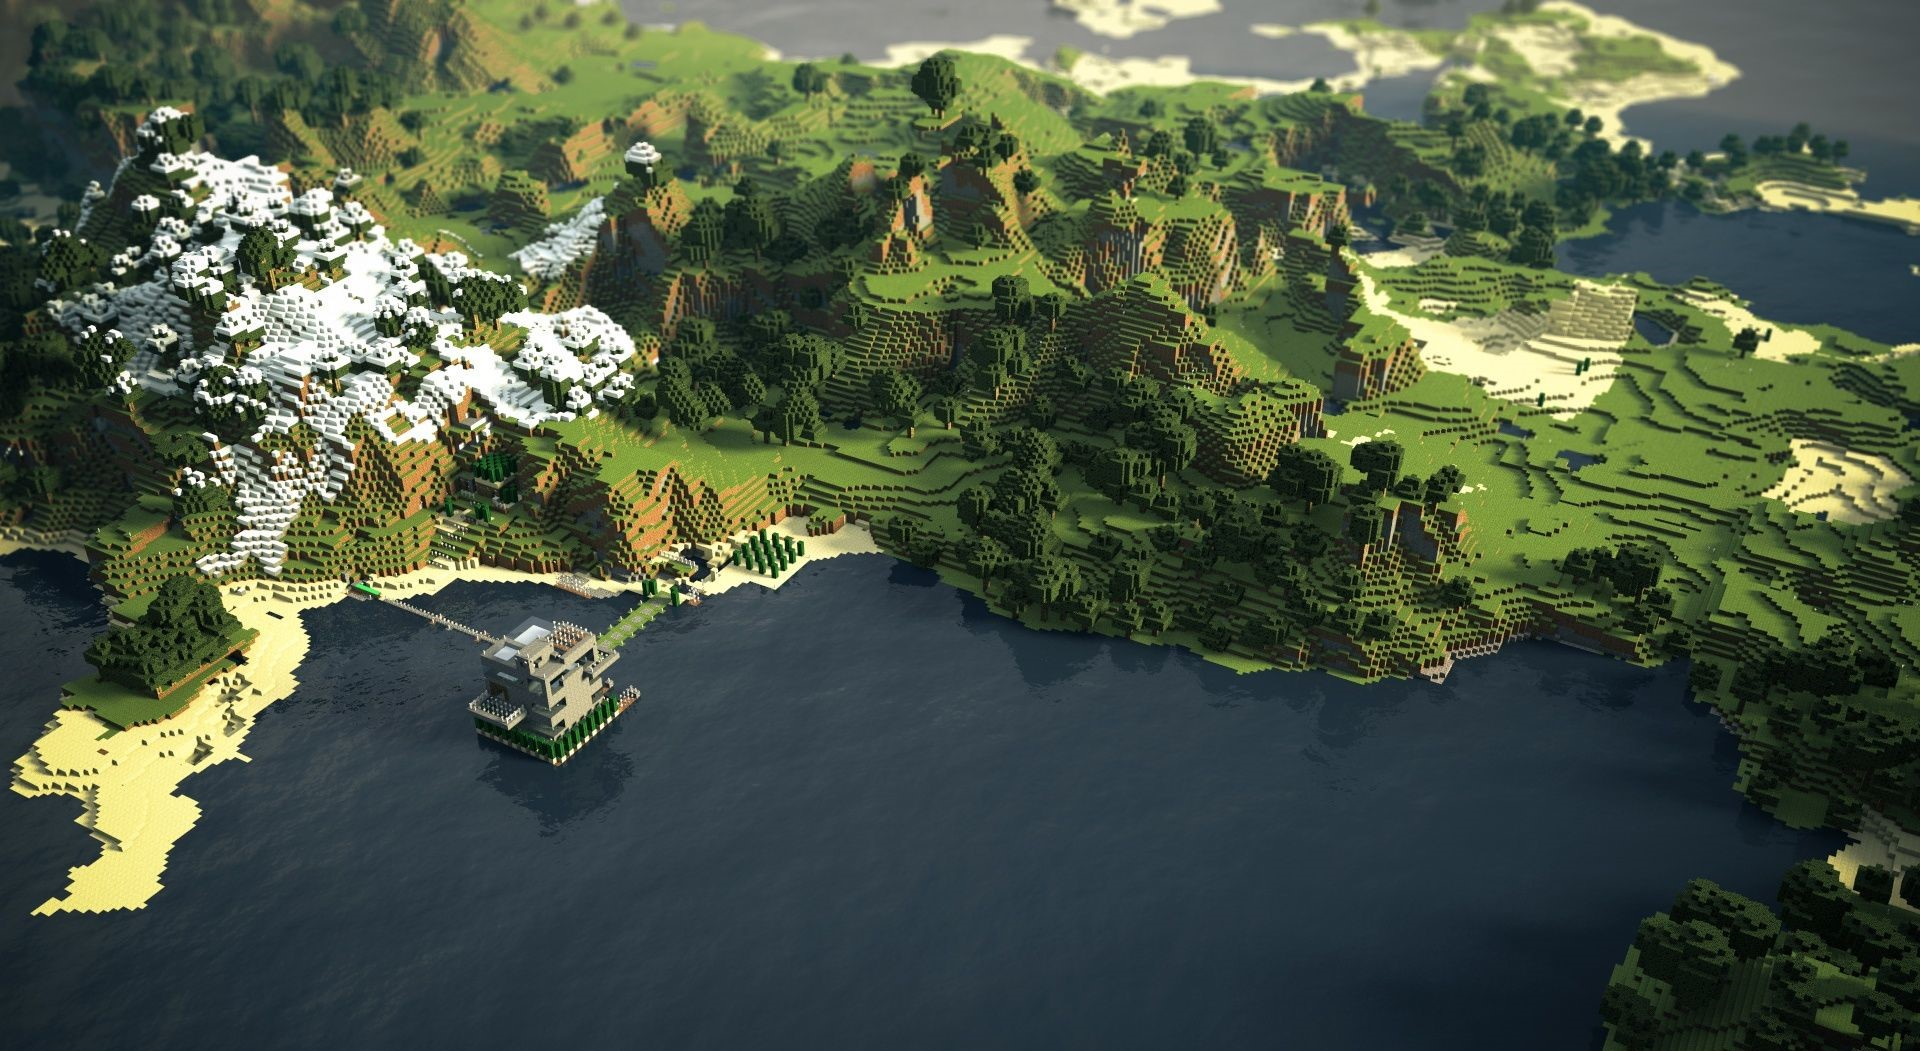
\includegraphics[width = 16cm]{figures/minecraft.jpg}
    \caption{An in-game screenshot of \textit{Minecraft's} procedurally generated environment, improved with a graphics enhancing mod.}
    \label{fig:minecraft}
\end{figure}

\textit{Perlin noise} proves once again how reliable the algorithm is. Minecraft uses a custom version of \textit{3D Perlin Noise} to generate all the blocks that make up the game world. Initially, only basic stone blocks are generated, defining the complete outline of the terrain, along with rivers and water masses at certain height levels. Next, all the caves are generated using an algorithm called \textit{Perlin worm}, which will be covered later on. Also at this step, different biomes are applied to map locations, radically changing the color palette, flora and fauna of the zones. Following this, minable ores are added to the game world, filling up the barren caves and underground world, creating one of the core gameplay elements of the game. At the end, the so called \textit{decoration elements} are added, which consist of trees, grass, animals and even structures, which are generated with stricter rulesets. The player can even input a custom \textit{seed}, that will always generate the same world, allowing for social elements, like sharing these character strings with other people, to enjoy the same landscapes, or pursuing the best procedurally generated level that the game's community has ever seen. \\

Hello Games' \textit{No Man's Sky} is another great example of a game that uses procedural generation heavily. Players can explore a whole virtual universe, with planets and moons that revolve around a sun, creating cycles of day and night, asteroids, even multiple solar systems and also cosmic phenomena. To be more precises, there are more than \(2^{64}\) planets, ready to be explored, filled with destructible terrain, computer generated alien flora and fauna, each with their own randomized names and stats. Such a feat would never be possible without procedural generation, because such a large number of assets would take a colossal amount of manual work, that would span over many years. The idea of space exploration and alien interaction gives the developers the freedom to configure the algorithms to output interesting, strange-looking characters and shapes, without worrying too much about realism but, for some reason, this doesn't take away from the game's immersion. With a virtual reality version of the game coming soon, Hello Games can expect a great success.

\subsection{Terrain}

One of the popular methods for terrain generation is modeling 3D surfaces using noise value maps. A function such as \textit{Perlin noise} can be used to deterministically obtain values between \([-1, 1]\) for each point of a 2D map. The result can be treated as a height map, and each value can be used to set the height coordinate of a 3D mesh, in order to alter its aspect and create an object that resembles a terrain outline, with mountains, fields and valleys. This is not enough to obtain realistic terrain, because at this stage, the result will look more like 3D sinusoidal waves. A well-known method used for adding details such as bumps, ridges and rocks to the map is \textit{noise layering}. By using what are usually called \textit{octaves}, we can stack multiple noise maps on top of another, each with different \textit{frequencies} and \textit{amplitudes}, in order to build the final result. Representing the noise map as a 2D graph, the wave-like structure of the values can be observed and some alteration options arise. Firstly, we can modify the \textit{frequency} of the noise, in order to create more waves, thus more detail, by introducing a variable called \textit{lacunarity}, that controls how much the frequency increases when adding successive octaves. A simple formula that can be used for \textit{frequency} is \(frequency=lacunarity^n, n=octave\), with a recommended value for the \textit{lacunarity} of $\approx$2. Secondly, we can also influence how much these details influence the final result by controlling the \textit{amplitude}. Same as before, we can introduce a variable called \textit{persistence}, adjusting how low or high is the influence of a certain octave over the final noise map. In order to achieve this, such a formula is used: \(amplitude = persistence^n, n=octave\), with a recommended value for the \textit{persistence} of $\approx$0.5. To better understand and visualize these concepts, please refer to Figure \ref{fig:terrainGraph}.\\

\begin{figure}[htp]
    \centering
    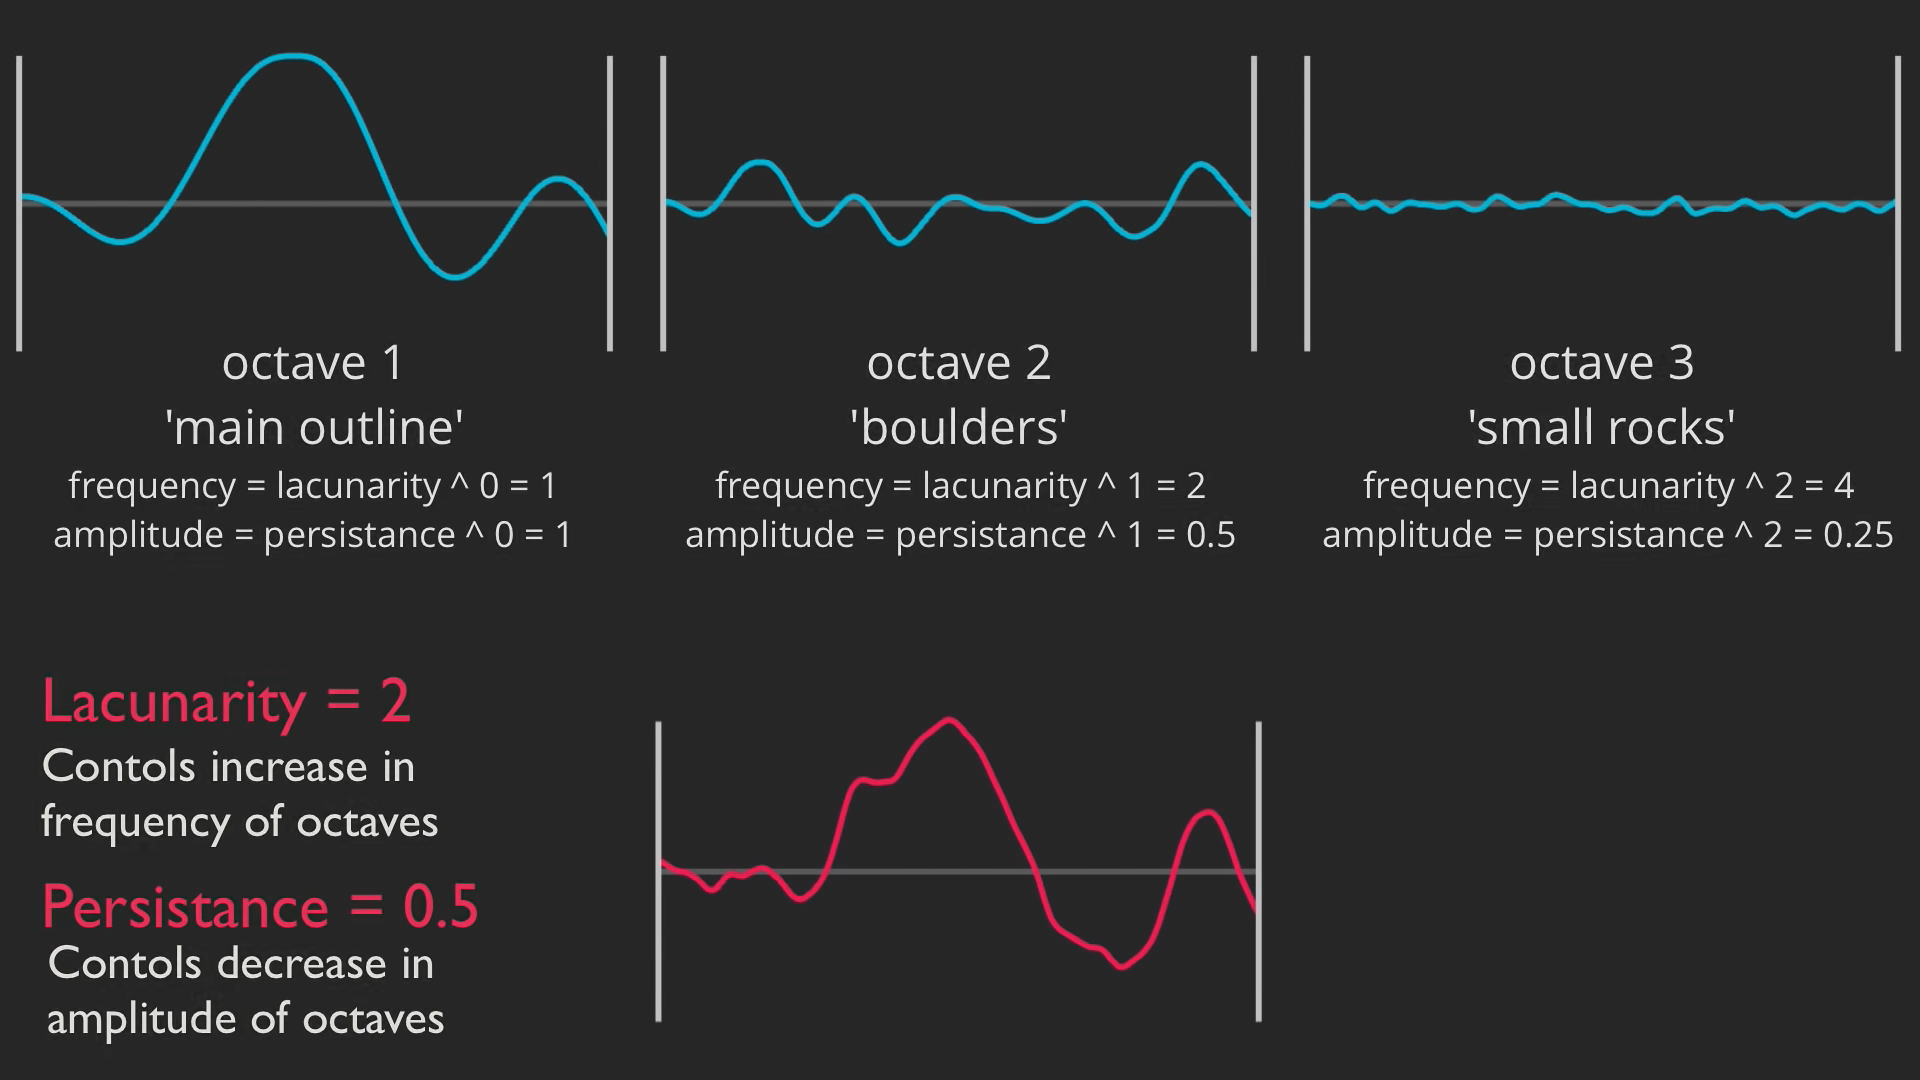
\includegraphics[width = 16cm]{figures/terrainGraph.png}
    \caption{A graphic example of how octaves (blue graphs), using frequency and amplitude, influence the result (red graph).}
    \cite{procGenIntro}
    \label{fig:terrainGraph}
\end{figure}

A type of noise similar to \textit{Perlin noise}, called \textit{value noise}, can be used to create digital terrain from real-world height maps. For example, using tools like \textit{Tangram Heightmapper}, one can obtain accurate height maps for locations all over the world. Analyzing the map by going pixel by pixel can give us information about the minimum and maximum \textit{grayscale} values, which in turn can be used to map all the values to a range suitable for our operations, for example \([-1, 1]\). Then, the procedure is the same as the one previously discussed\cite{parberry2014designer}.\\

The height maps can be further processed by applying artificial image filters, such as smoothing, or blurring, that can improve them by a certain degree, but to really obtain some great results, powerful algorithms that simulate \textit{thermal} or \textit{hydraulic erosion}, which will be discussed later on, are used. These algorithms are the ones that add the most realism to a scene. What \textit{thermal erosion} does is distribute "material" from higher values to lower values, until a satisfying slope angle is obtained. \textit{Hydraulic erosion} simulates rainfall by calculating how much \textit{sediment} is carried down a mountain or a hill, subtracting values on each iteration.\cite{smelik2009survey}. 

\subsection{Caves, dungeons and mazes}

In some games, it is not always enough to just let the player wander around on the surface. A sense of verticality is much needed for some worlds, especially the procedurally generated ones. Structures like cave systems, ravines and dungeons (as seen in \textit{Minecraft}), add completely new gameplay elements. For some other genres, mazes add the element of tension, surprise and excitement. Intuitively, one can attempt to use \textit{3D Perlin noise}, but the results can end up underwhelming. Among successful generation methods are \textit{cellular automata} and \textit{Perlin worms}. \textit{Cellular automata} is a grid-like system with spaces occupied by what we will call \textit{cells}, that follow the next rules:
\begin{gather*}
    (1)\;if\;a \;cell\;has\;fewer\;than\;two\;neighbours,\;it\;dies;\\
    (2)\;if\;a \;cell\;has\;two\;or\;three\;neighbours,\;it\;lives\;on\;to\;the\;next\;generation;\\
    (3)\;if\;a \;cell\;has\;more\;than\;three\;neighbours,\;it\;dies;\\
    (4)\;if\;a\;dead\;cell\;is\;surrounded\;by\;exactly\;three\;cells,\;it\;gets\;revived;
\end{gather*}
By experimenting with starting configurations of cells, we can simulate a high amount of generations and mark as visited each space of the grid that has had a cell at one point. Cells will move around the grid, and eventually, they will stabilise. The results are complex grids that can now resemble cave systems, or dungeons (see Figure \ref{fig:cellularAutomata}). For maze generation, the starting configurations have to be crafted and thought of beforehand. \textit{Perlin worm} is a method that uses three octaves of \textit{Perlin noise}, using each one to compute an x-y-z values tuple. Choosing a starting point in a 3D space, one can run many iterations, generating at each step new values for the octaves, thus receiving new coordinates. Following these coordinates yield great results in term of cave systems, the best example being, again, the game \textit{Minecraft}, which we already covered. 

\begin{figure}[htp]
    \centering
    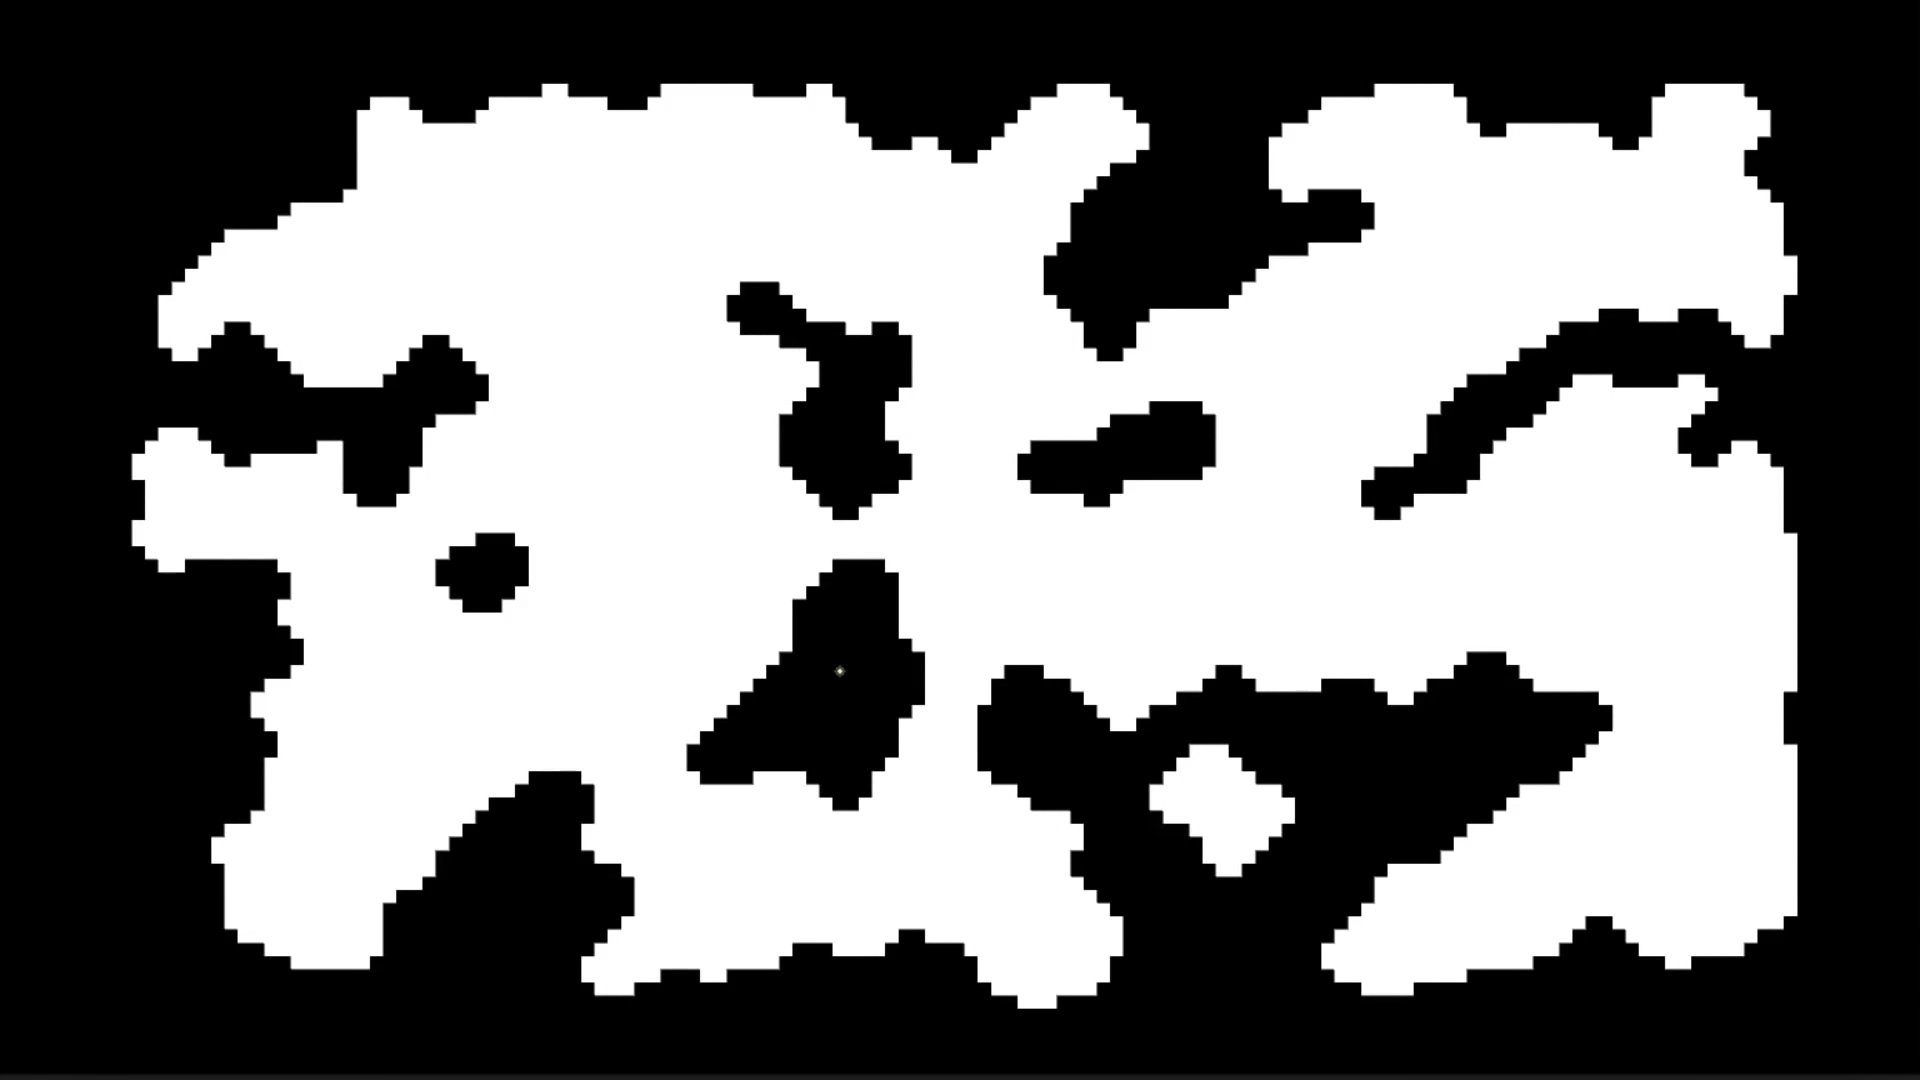
\includegraphics[width = 16cm]{figures/cellularAutomata.png}
    \caption{A 2D cave system generated using the \textit{cellular automata} algorithm.}
    \cite{procCaveGen}
    \label{fig:cellularAutomata}
\end{figure}

\subsection{Bodies of water}

In a 2009 paper called \textit{A Survey of Procedural Methods for Terrain Modelling}\cite{smelik2009survey}, there are some techniques of water body generation discussed. The process of generating \textbf{rivers} usually happens during or after the creation of the height map. A "single, straight river" is recursively subdivided, resulting in a complex network of streams, all across the map. The climate of the area can also influence some particularities of the river, the soil etc. Another interesting way of generating rivers is placing a pair of \textit{ridge particles} and moving them away from each other in multiple iterations. After each iteration, a \textit{Gaussian curve} is drawn between the points. Finally, the actual river is created by placing water-physics particles, that can be simulated to flow down the formed ridges, fairly similar to an erosion simulation. \textbf{Seas and oceans} on the other hand, are quickly set up by attributing a fixed water level, for example 0m, or by using a \textit{flooding algorithm}, starting from the lowest point on the map up until a decided end point. Unfortunately, \textbf{lakes} and \textbf{coastal features} have not received much attention, and their generation is usually "not considered at all".

\subsection{Biomes}

\textbf{Biomes} can be defined as regions of land with specific characteristics. Some examples of biomes are arid, semi-arid, semi-humid, humid etc. There are numerous variations of biomes and usually, in games that implement them, the decision stands from a design point. One basic solution to integrating biomes into your game is color-coding the terrain by the heights. For example, if the height values are in the range of \([0, 1]\), the regions between 0 and 0.4 could be blue, standing for water, or the regions between 0.9 to 1 could be white, giving the impression of snow covered mountain peaks. While being an accessible implementation of biomes, it is also bland and boring, because there is no variety, and there is a lot of repetition: bodies of water will always be surrounded by sand, mountains by forests etc. One method that can improve the overall aspect of the generated terrain is creating a custom shader, that applies a texture for each specified region, and blends it with the surrounding ones, creating a seamless surface.\\

One more complex solution would be to generate two extra noise maps, one for humidity and one for temperature. Each of the maps can be generated with multiple layers, for increased detail and diversity. Using a combination of the two maps, different algorithms can be used to generate the terrain, obtaining realistic biomes. If designing a game with "infinite" terrain generation, there is a lot more "artistic freedom", and how the biomes are actually distributed is not very important, if not striving for realistic environments. When creating maps that come close to a 1:1 scale with our own planet, things get complicated. There are some attempts such as this one \cite{biomes}, where the developer tries to compute temperature and precipitation maps "based on essential principles of Earth's climate", even going to the extent of analyzing wind currents and compensating for the \textit{Coriolis effect}. Even after all these improvements, the transitions can still be rough and artificial-looking. One last effort to make things right is to implement a \textit{pressure map} that can yield more natural results, with smoother transitions and a realistic feel to the obtained climates.

\subsection{Vegetation}

A big challenge in game development is populating vast areas with small vegetation, grass and trees. Even though placing each asset by hand can result in a more visually appealing result, the process is time consuming. In the game industry, time is an essential resource, therefore there is a lot of research ongoing on this topic. Methods of efficiently placing high number of foliage and trees are already present in most of the 3D computer graphics software and game engines, in form of brushes that can be used to "paint" on the game world. In the area of procedural generation, objects occurring naturally in our world are probably the most studied, mostly because of the interest in theoretical biology, as stated in \cite{freiknecht2017survey}. Hungarian scientists Prusinkiewicz and Lindenmayer were among the first to start researching methods to describe the structure of plants using mathematical approaches. They suggested using a grammar, called \textit{L-Systems (Lindenmayer Systems)}. In order to better visualize the method, a graphical representation in form of a 2D grid, seen in Figure \ref{fig:turtleModel}, often called the \textit{turtle model}, can be used, with the following rules defined:
\begin{gather*}
    F->move\;one\;step\;forward,\;drawing\;a\;line;\\
    f->move\;one\;step\;forward\;without\;drawing\;a\;line;\\
    +->turn\;right\;by\;\delta\;degrees;\\
    ->turn\;left\;by\;\delta\;degrees;\\
    \cite{freiknecht2017survey}
\end{gather*}

\begin{figure}[htp]
    \centering
    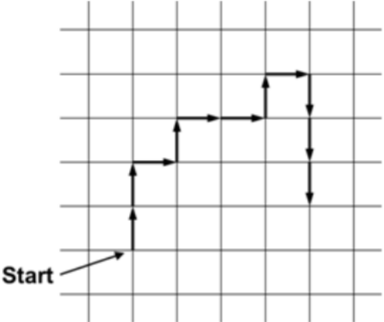
\includegraphics[width = 8cm]{figures/turtleModel.png}
    \caption{A structure produced using the \textit{turtle model}, where the starting point is \((1, 1)\), and \(\delta = 90^{\circ}\), corresponding to the word \textbf{FF-F+F-FF+F-F-FFF}.}
    \cite{freiknecht2017survey}
    \label{fig:turtleModel}
\end{figure}

Based on this principle, 2D plants can efficiently be generated, with an example shown in Figure \ref{fig:plants}. Extending this method with new rules and notions such as "\textit{pitch up}, \textit{pitch down}, \textit{roll up} and \textit{roll down}" allows the grammar to produce 3D models as well\cite{freiknecht2017survey}. Denser plants like bushes can benefit from additional properties such as \textit{branch width}, and using variables that adjust the \textit{color}, for instance, helps with styling the results.

\begin{figure}[htp]
    \centering
    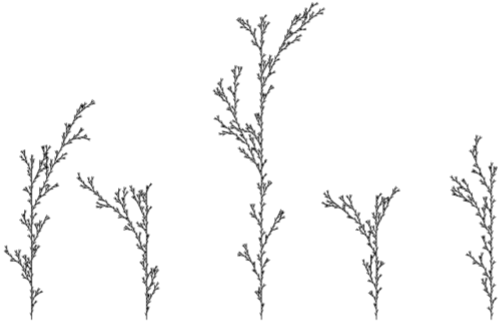
\includegraphics[width = 12cm]{figures/plants.png}
    \caption{2D plants generated using the \textit{L-System}, proposed by Prusinkiewicz and Lindenmayer.}
    \cite{freiknecht2017survey}
    \label{fig:plants}
\end{figure}

\subsection{Roads and cities}

Some games, especially the ones in the \textit{city-building} genre, are built with road generation systems at their core. Traffic infrastructure is an essential thing to manage in such games, from a gameplay perspective, thus the need of powerful, resource-light algorithms is present. There is no need to focus on air or sea traffic, since naive implementations are satisfactory, most of the times. Ilangovan proposes in his thesis \cite{ilangovan2009procedural} a method of generation that starts with the highways, the main entry-points in the map. Giving the generator groups of \textit{junction points}, a basic layout of the road system can be created, acting as the main artery from which other streets will branch out. Road creating tools that can allow players to draw their own road meshes on the map can be implemented using \textit{spline interpolations}.\\

Another important aspect of \textit{city-building} games are the buildings, which have to be placed on the plots defined by the areas enclosed by streets, or along the streets, in plots of fixed dimensions. The buildings and objects such as street lamps, hydrants and cars are distributed randomly, following set rules. The assets can be also be procedurally generated, with algorithms able to do this already having been discussed (with the necessary modifications, of course). The simplest way is to have them already modeled beforehand, manually, then deterministically alter their rotation, size and location, based on different factors.

\section{Related algorithms}

\subsection{Planets}

Generating planets shares a lot of common ground with terrain generation. The idea is very similar: generate a noise map and model a spherical mesh based on it. The difficult part is trying to create different \textit{levels of detail (LOD)}, which is a big part in optimizing video games with complex 3D objects. \textit{LOD switching} implementations are usually designed to work on surfaces based on planes. When working on unorthodox surfaces, clever solutions have to be found. One is to actually create a sphere by "inflating" a cube, until there are no more sharp edges. Even though calculating \textit{normals} will be harder, the overall difficulty of the task will be lower, due to the fact that a sphere can now be thought of as 8 separate bent planes, stuck together. Also, the \textit{triangle count} will decrease, and will be more easily controlled, further increasing the performance of the application, whereas when working with a sphere, the number of triangles would increase rapidly near the two poles. Martin Kahoun talks in \cite{kahoun2010procedural} about a method that applies \textit{geometry clipmaps} to the elevation map, but the results are not good enough, because the \textit{LOD} would be controlled purely based on distance, and other factors that make a good implementation would miss.

\subsection{Marching cubes}

The \textit{marching cubes} algorithm has many uses, but one of the most interesting ones is in terrain generation. Consider we have a region of 3D space, chosen randomly. We can sample points at regular intervals, as seen in Figure \ref{fig:marchingCubes}, and feed their x-y-z coordinates, one by one, into a deterministic function that outputs a single value as a result. Computing the minimum and maximum of all the obtained values, we can create a \textit{spectrum}, used in later steps to control the \textit{surface level}.  

\begin{figure}[htp]
    \centering
    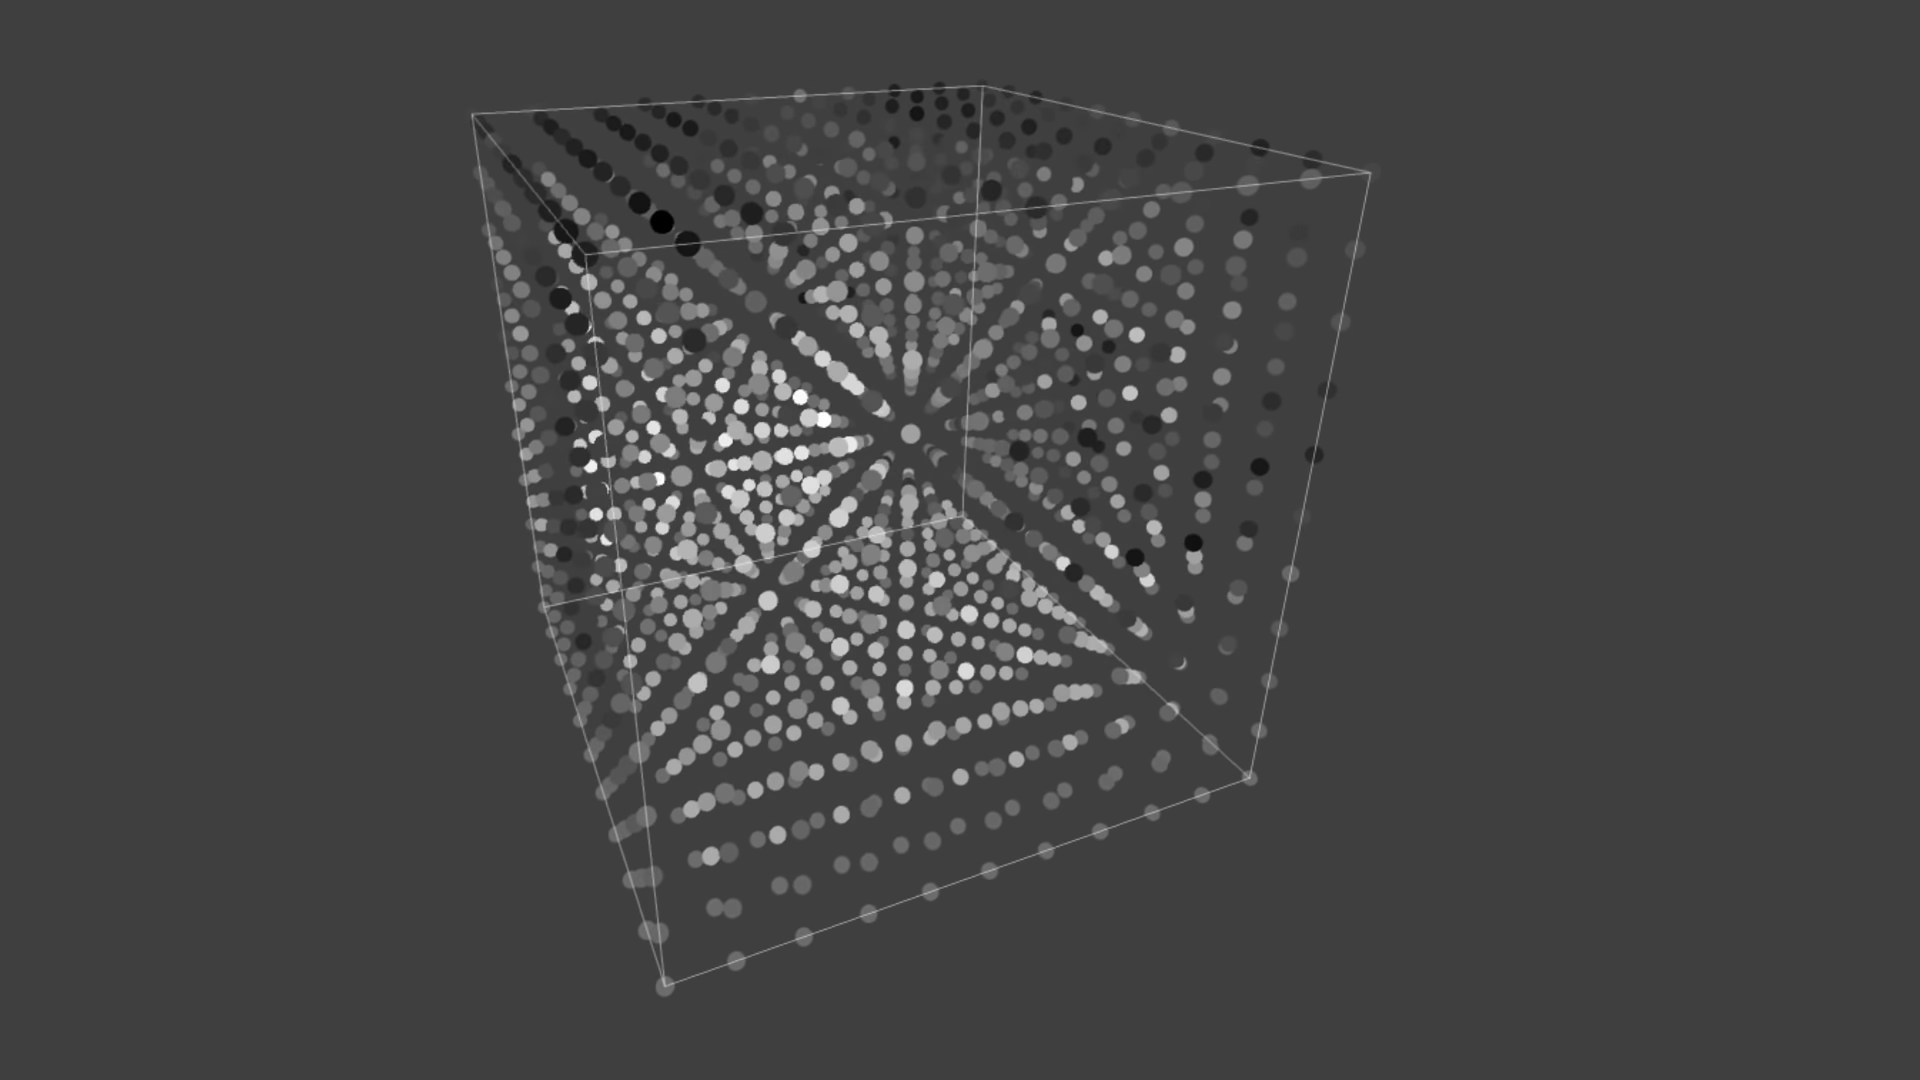
\includegraphics[width = 11cm]{figures/marchingCubes.png}
    \caption{A cube with multiple values sampled as points, at regular intervals.}
    \cite{marchingCubes}
    \label{fig:marchingCubes}
\end{figure}

Let us suppose we set the \textit{surface level}, which can take values from \([-34, 16]\), to a value of \(-0.2\). All the points with coordinates that evaluate to a value below \(-0.2\) will be hidden, and not be taken into consideration when building the final result. The goal of the \textit{marching cubes} algorithm is to use the remaining, visible points to form triangles, which in turn will create the final 3D object, as seen in Figure \ref{fig:marchingCubesResult}. The method is described in depth in the paper \textit{MARCHING CUBES: A HIGH RESOLUTION 3D SURFACE CONSTRUCTION ALGORITHM}\cite{lorensen1987marching}, from 1987, in which the author also describes numerous applications, especially in the medical field.

\begin{figure}[htp]
    \centering
    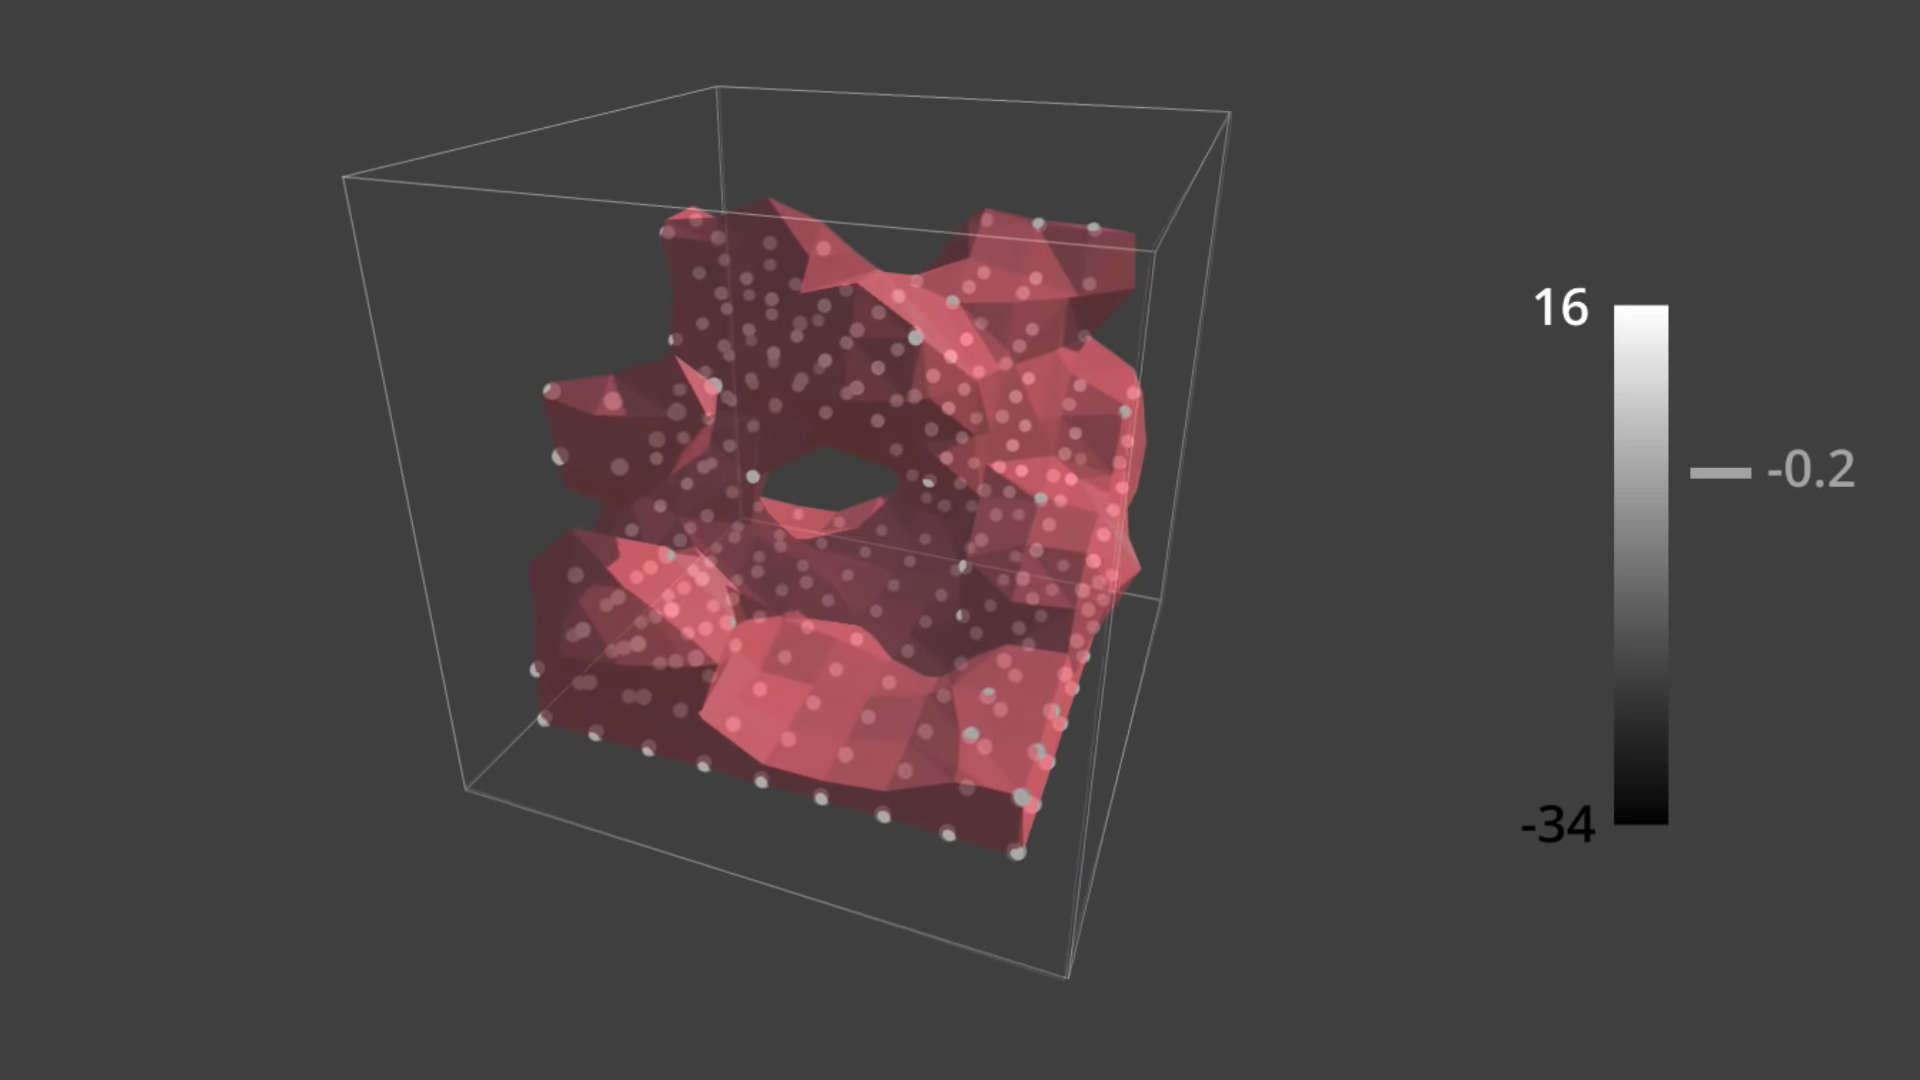
\includegraphics[width = 11cm]{figures/marchingCubesResult.png}
    \caption{A cube in which only the points that evaluate above the selected value are shown, forming triangles and thus the final shape.}
    \cite{marchingCubes}
    \label{fig:marchingCubesResult}
\end{figure}

\section{Simulations}

\subsection{Overview}

Some projects require a finer level of detail, and a higher level of realism. For example, a generated terrain will often miss "the final touch". In order to solve the problem and obtain a result that is almost indistinguishable from its real-life counterpart, most developers implement certain algorithms, or use software that can run simulations of real phenomena, such as \textit{thermal erosion}, \textit{hydraulic erosion} or \textit{clouds}. Also, when programming AI for flocks of birds, schools of fish or other groups of animals, this behaviour can be replicated with techniques such as the so called \textit{boids}.

\subsection{Erosion}

\textit{Thermal erosion} and \textit{hydraulic erosion} are natural phenomena that are highly studied in the field of computer graphics. A great paper that describes these and also offers an implementation that heavily utilizes the GPU, is \textit{Fast Hydraulic and Thermal Erosion on the GPU}, written in 2011 by Balasz Jako\cite{jako2011fast}. \textit{Thermal erosion} is described as hard surfaces that crack in smaller pieces, that move down to lower areas, due to gravity. The cause is the changing temperature, happening due to "the alternation of the hot Sun and the cold night air". \textit{Hydraulic erosion} is the result of rainfall and rivers dissolving land material and carrying it to different locations, where the \textit{sediment} is deposited. Due to the increased power of modern GPUs, physics based models are used to create fluid simulations, marking one way of achieving virtual erosion. Another way is using advanced particle systems, that are programmed to hit the ground, which is considered a 2D grid, and substract a certain value from the affected points, then calculate the velocity of the particles, to simulate them down-hill. All of this can be done in real-time, allowing the user to observe at each step the different results the algorithms produce. A side-by-side comparison between terrain generated using a noise map, with the aid of \textit{Perlin noise}, and the same terrain, enhanced by simulating \textit{hydraulic erosion}, can be seen in Figure \ref{fig:hydraulicErosion}.

\begin{figure}[htp]
    \centering
    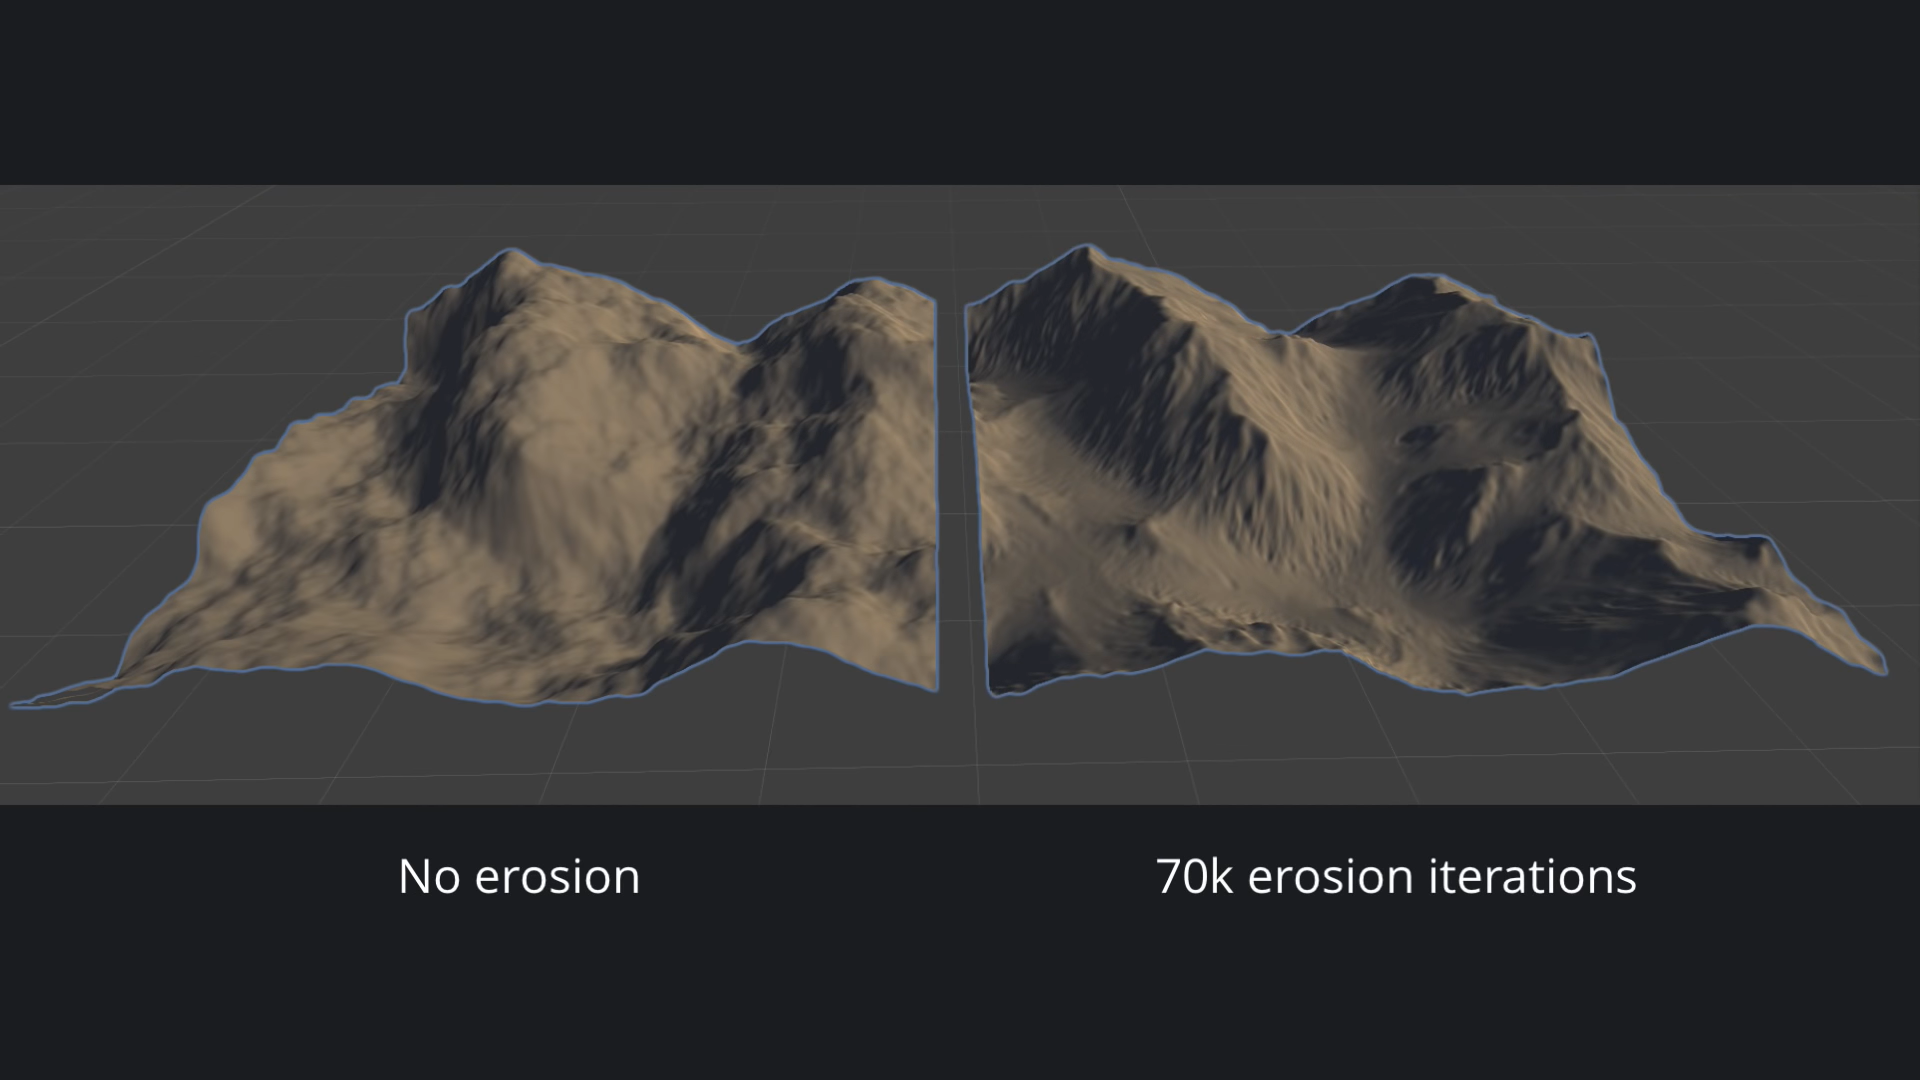
\includegraphics[width = 16cm]{figures/hydraulicErosion.png}
    \caption{A side-by-side comparison between a standard, procedurally generated terrain, and a terrain affected by 70.000 iterations of hydraulic erosion, all simulated in $\approx$3 seconds.}
    \cite{hydraulicErosion}
    \label{fig:hydraulicErosion}
\end{figure}

\subsection{Clouds}

In video games, \textit{skyboxes} are one of the oldest tricks in the book. Developers enclose all the game area in a cube, and using a technique called \textit{cube mapping}, they project textures depicting the sky and unreachable landscapes, on all the interior faces of the cube\cite{skyboxWiki}. This way, the playable area is actually faked to look much greater than it actually is. A benefit of using this method is better performance, since the distant objects do not have to be real, modeled 3D objects that are actually rendered on the screen dynamically, significantly decreasing the need of high draw distances. Older games deal with clouds by "painting" them directly on the \textit{skybox}, as hand-crafted or procedurally generated textures\cite{roden2005clouds}. Their movement can be simulated by rotating the textures, or slightly altering the \textit{UV mapping}. Unfortunately, for today's standards, this is just not good enough anymore.\\

State-of-the-art techniques involve generating \textit{clouds} that have actual volume, and follow real-world physics principles\cite{ebert1997volumetric}. One popular method of generating cloud shapes is using \textit{Worley noise}. To understand this algorithm, let us suppose we have a square, in which we scatter points randomly. In order to compute the noise map, we set the value of each pixel inside the square to the distance between that pixel's position and the nearest randomly placed point, mapped to a suitable range of values, such as \([-1, 1]\). Using a slightly altered version of this function, we can generate 3D noise maps, in which the resemblance to clouds is already seen. What really gives the realistic feel to \textit{volumetric clouds} is the ability of light to pass through them, with the amount of light controlled by the density of the clouds. Dynamic shadows can be cast on the surface of the game world, and lighting can change in real-time, in relation to the clouds; some developers also go to the extent of programming the so called \textit{god rays} effect\cite{godraysWiki}. The biggest downside is the fact that this technique is very taxing on computer resources and, due to the fact that a powerful GPU is required, not many players end up enjoying the beautiful virtual worlds, filled with \textit{volumetric clouds} (see Figure \ref{fig:clouds}).

\begin{figure}[htp]
    \centering
    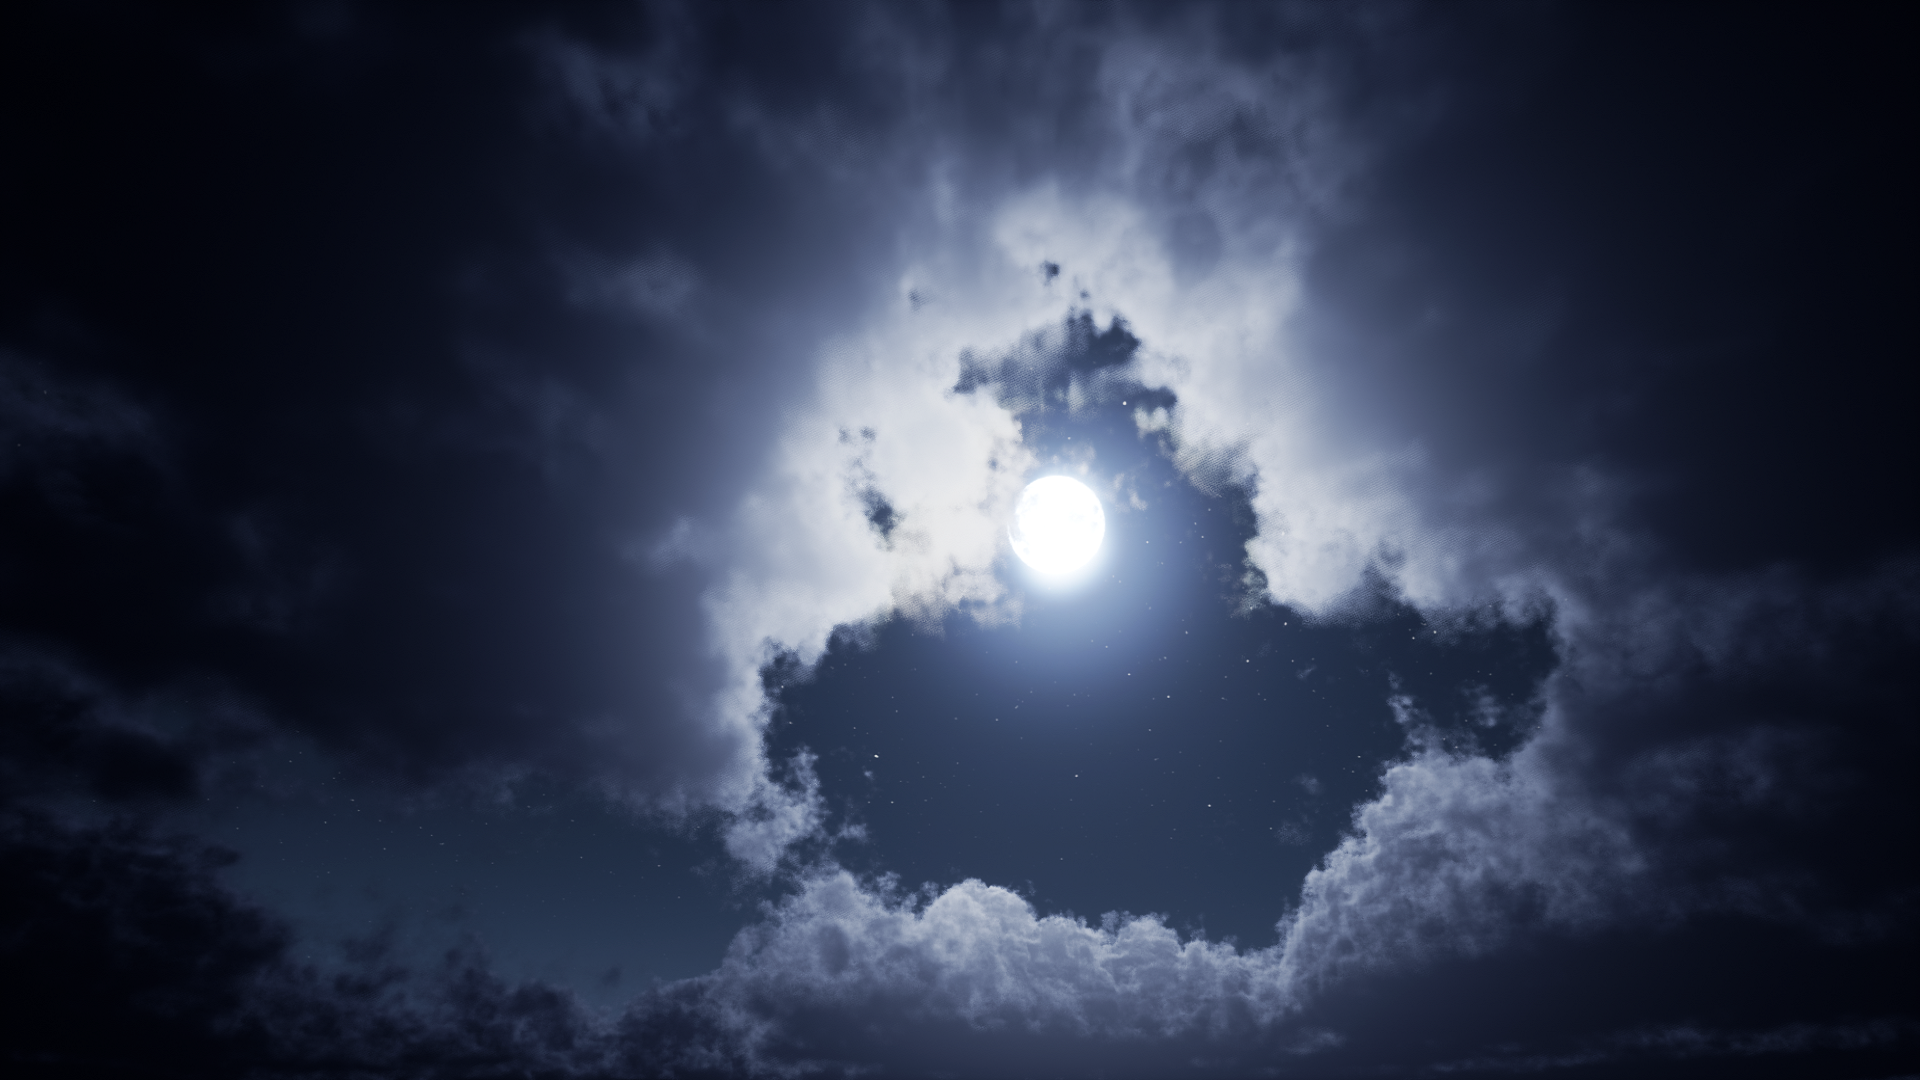
\includegraphics[width = 16cm]{figures/clouds.png}
    \caption{A screenshot of an in-game scene showcasing a dynamic sky system with \textit{volumetric clouds}.}
    \cite{dynamicSky}
    \label{fig:clouds}
\end{figure}

\subsection{Boids}

Programming AI for \textit{non-playable characters} (NPCs) can sometimes prove to be a challenging task, and some smaller developers resort to 3rd party libraries, or implement naive solutions. Group behaviour of animals is a feature that not many games showcase, but in some instances (e.g., an underwater level), things like schools of fish that interact with the player are a big gameplay or atmospheric element. A well-known technique of generating a group of animals, in which each one acknowledges the existence of another, is called \textit{boids}, short for "bird-oid" objects, described thoroughly in \textit{Flocks, Herds, and Schools: A Distributed Behavioral Model}\cite{reynolds1987flocks}, published in 1987 by Craig W. Reynolds. A \textit{boid}, that in a basic graphic representation can conveniently be denoted by a small square or triangle, has to follow some rules. These rules are not strict, offering some degree of flexibility, in order to obtain the specific result that one wants to observe. The first rules says that one \textit{boid} has a fixed field of view, that helps him steer away from other directly incoming \textit{boids}, in order to avoid crashing (behaviour known as \textit{separation}). The second and a more important rule says that \textit{boids} have to correct their velocity by trying to match the velocity of nearby passing \textit{boids} (behaviour known as \textit{alignment}). Last but not least, the final rule states that every \textit{boid} has to "gravitate" towards the center of mass of the nearest formed group (behaviour known as \textit{cohesion}). Simulations based on this algorithm can come extremely close to the real-life structure and behaviour of bird flocks, fish schools or other animals that group up, especially if done in a 3D environment, with convincing visual models.